\section{整组随机化的误差}
\label{sec:mcerr-replication}

有些采样方法一次产生一组彼此相关的点：每个点单独看都服从目标分布，但点与点之间被有意安排，使整组覆盖得更均匀。第~\ref{chap:variance-reduction}章的拉丁超立方采样与随机化准Monte Carlo都属于这一类。这样的组内平均无偏，方差却不能用独立公式计算，同一组点的样本方差也不反映它。办法是把整组当作一个观测单位，独立地重复整个构造。

\paragraph{整体平移的网格}
用一个最简单的构造说明。目标仍是$I=\int_0^1\mathrm{e}^{u}\,\mathrm{d}u$。取$n$个等距点$a_i=(i-1)/n$，$i=1,\dots,n$，再取一个$\Delta\sim\operatorname{Unif}(0,1)$，把所有点一起平移并按模$1$回绕：
\[
 U_i=(a_i+\Delta)\bmod1 .
\]
对固定的$a\in[0,1)$与$s\in[0,1]$，使$(a+\Delta)\bmod1\leq s$的$\Delta$构成$[0,1)$中总长度为$s$的一个或两个区间，所以每个$U_i$都服从$\operatorname{Unif}(0,1)$。由第~\ref{sec:mcerr-estimator}节，组平均
\[
 Q=\frac1n\sum_{i=1}^{n}f(U_i)
\]
是$I$的无偏估计。但这些点完全不独立：知道一个点，就知道了整组。

$n=4$时，组平均只依赖$\Delta'=\Delta\bmod\tfrac14$：四个点就是$\Delta'+j/4$，$j=0,1,2,3$。对$f(u)=\mathrm{e}^{u}$，等比求和给出
\begin{equation}
 Q=\frac{\mathrm{e}^{\Delta'}}{4}\sum_{j=0}^{3}\mathrm{e}^{j/4}=c\,\mathrm{e}^{\Delta'},\qquad c=\frac{\mathrm{e}-1}{4(\mathrm{e}^{1/4}-1)}=1.5124 .
 \label{eq:mcerr-shift-q}
\end{equation}
四个点均匀地分布在$[0,1)$上，相互弥补，$\operatorname{Var}(Q)=0.01536$；同样四个独立均匀点的平均，方差是$\sigma_f^{2}/4=0.0605$，大了约四倍。组内的依赖正是精度提高的来源，也正是它使独立公式失效。

\subsection{组间方差}
\label{sec:mcerr-between-var}

固定每组点数$n$，用独立的随机数重复同一个随机化规则$R$次，得到组估计$Q_1,\dots,Q_R$。它们独立同分布，每一个都是一次完整构造的结果。

\begin{theorem}[组间方差估计]
\label{thm:mcerr-between-var}
设$Q_1,\dots,Q_R$独立同分布，$\mathbb{E}[Q_1]=I$，$\mathbb{E}[Q_1^{2}]<\infty$，$R\geq2$。令
\begin{equation}
 \bar{Q}=\frac1R\sum_{r=1}^{R}Q_r,\qquad s_Q^{2}=\frac{1}{R-1}\sum_{r=1}^{R}\bigl(Q_r-\bar{Q}\bigr)^{2} .
 \label{eq:mcerr-between}
\end{equation}
则$\mathbb{E}[\bar{Q}]=I$，并且
\begin{equation}
 \operatorname{Var}(\bar{Q})=\frac{\operatorname{Var}(Q_1)}{R},\qquad \mathbb{E}\Bigl[\frac{s_Q^{2}}{R}\Bigr]=\operatorname{Var}(\bar{Q}) .
 \label{eq:mcerr-between-unbiased}
\end{equation}
\end{theorem}

\begin{proof}
前两条是独立同分布变量平均的期望与方差，与定理~\ref{thm:mcerr-iid-bound}的证明相同。记$v=\operatorname{Var}(Q_1)$。把每一项写成$Q_r-\bar{Q}=(Q_r-I)-(\bar{Q}-I)$，展开平方和，并利用$\sum_r(Q_r-I)=R(\bar{Q}-I)$，
\[
 \sum_{r=1}^{R}\bigl(Q_r-\bar{Q}\bigr)^{2}=\sum_{r=1}^{R}(Q_r-I)^{2}-R\,(\bar{Q}-I)^{2} .
\]
取期望，第一项为$Rv$，第二项为$R\cdot v/R=v$，所以
\[
 \mathbb{E}\Bigl[\sum_{r=1}^{R}\bigl(Q_r-\bar{Q}\bigr)^{2}\Bigr]=(R-1)\,v .
\]
除以$R-1$得$\mathbb{E}[s_Q^{2}]=v$，再除以$R$即得结论。
\end{proof}

定理只用到组与组之间的独立，对组内点的依赖没有任何要求。这正是需要的分工：组内怎样安排由设计决定，误差由组间的波动来度量。反过来，把$nR$个点混在一起求样本方差再除以$nR$，相当于假装这些点彼此独立，没有依据。

\paragraph{四组的计算}
取$n=4$，$R=4$，四次平移为
\[
 \Delta_1=0.37,\quad \Delta_2=0.81,\quad \Delta_3=0.19,\quad \Delta_4=0.64 ,
\]
如图~\ref{fig:mcerr-group-shift}(a)。按模$\tfrac14$约化，$\Delta'$依次为$0.12,0.06,0.19,0.14$。代入式~\eqref{eq:mcerr-shift-q}，
\[
 Q_1=1.7053,\quad Q_2=1.6060,\quad Q_3=1.8289,\quad Q_4=1.7397 .
\]
总平均为$\bar{Q}=1.7200$，与$I=1.7183$相差$0.0017$。各组与总平均的差是$-0.0147,-0.1140,0.1089,0.0198$，由式~\eqref{eq:mcerr-between}，
\[
 s_Q^{2}=0.008491,\qquad \frac{s_Q^{2}}{R}=0.002123,\qquad \sqrt{s_Q^{2}/R}=0.0461 .
\]
真实的$\operatorname{Var}(\bar{Q})=0.01536/4=0.00384$，标准差为$0.0620$；只有四组时，估计值$0.0461$偏小，但这是随机波动，不是系统偏差。

若把$16$个函数值当作独立样本，它们的样本方差为$0.2483$，除以$16$得$0.01552$，标准误差$0.1246$，是真实值的两倍。它实际上估计的是$16$个独立点的方差$\sigma_f^{2}/16$，完全没有反映网格带来的改进。这里组内点相互弥补，独立公式高估了误差；若组内点彼此相似，例如一段链记录，独立公式就会低估误差。两个方向的错误都来自同一个原因：用组内的离散程度代替了组间的波动。

图~\ref{fig:mcerr-group-shift}(b)把整个实验（每次$R=4$组）重复$5000$次。正确估计$s_Q^{2}/R$的平均为$0.00382$，与真实值$0.00384$一致，但分布很宽，因为每次只有四个组估计；混合估计集中在$0.0159$附近，稳定地错了四倍。

\begin{BookInlineFigure}
 \centering
 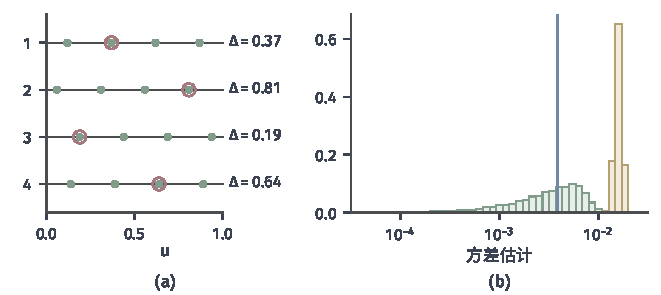
\includegraphics[width=112mm]{figures/07-probability/08-sampling-and-integration/matplotlib/mcerr-group-shift/figure.pdf}
 \caption{整体平移网格估计$\int_0^1\mathrm{e}^{u}\,\mathrm{d}u$，每组$n=4$点。(a)四组点（绿点），红圈为各组的平移量$\Delta_r$；(b)整个实验（$R=4$）重复$5000$次（种子$3133$）：绿色为$s_Q^{2}/R$的分布，黄色为把$16$个值当作独立样本的估计，蓝线为真实的$\operatorname{Var}(\bar{Q})=0.00384$，横轴为对数刻度。}
 \label{fig:mcerr-group-shift}
\end{BookInlineFigure}

\subsection{渐近误差区间}
\label{sec:mcerr-replication-interval}

组估计$Q_1,\dots,Q_R$是独立同分布的观测，第~\ref{sec:mcerr-asymptotic-interval}小节的结论可以原样搬过来，只是把“样本”换成“整组”，把样本数$N$换成重复数$R$。若$n$固定，$0<\operatorname{Var}(Q_1)<\infty$，则由定理~\ref{thm:mcerr-iid-clt}，$R\to\infty$时
\begin{equation}
 \frac{\sqrt{R}\,(\bar{Q}-I)}{s_Q}\xrightarrow{\mathrm{d}}\mathcal{N}(0,1) ,
 \label{eq:mcerr-replication-clt}
\end{equation}
区间$\bar{Q}\pm z\,s_Q/\sqrt{R}$的覆盖概率趋于$1-\alpha$。

上面的四组给出区间
\[
 1.7200\pm1.96\times0.0461=[1.6297,\,1.8103] ,
\]
包含$I$。但$R=4$离“$R\to\infty$”很远。由式~\eqref{eq:mcerr-shift-q}，$Q$是$\Delta'$的指数函数，取值在一个有界区间内，并不服从正态分布。用$20$万次重复实验（种子$3134$）估计，这个区间的实际覆盖概率在$R=4$时为$0.840$，$R=10$时为$0.917$，$R=30$时为$0.939$，$R=100$时为$0.947$。

对少量重复，常见的做法是把$z$换成自由度为$R-1$的t分布分位数，$R=4$时为$3.182$。若各组估计恰好服从正态分布，这能给出精确的覆盖概率；但组估计一般不是正态的，本例中这样做的覆盖概率是$0.929$，仍低于$0.95$。所以少量整组重复只能给出近似的误差范围，不提供有限样本下的精确覆盖保证。

这一节的结论可以概括为两条。第一，组内点边缘分布正确只保证无偏，不意味着它们彼此独立，组内的样本方差不衡量估计的误差。第二，独立重复的整组是误差估计的基本单位，误差区间的可靠程度由重复数$R$决定，而不是由总点数$nR$决定。第~\ref{chap:variance-reduction}章设计组内结构以减小$\operatorname{Var}(Q)$时，都按这里的方式估计误差。
